\documentclass{article}
\usepackage{../cs170}
\usepackage{physics}
\AtBeginDocument{\RenewCommandCopy\qty\SI}

\def\title{HW 11}

\begin{document}

\maketitle

\question{}

\begin{align}
  \lambda &= \qty{0}{\per\volt} \\
  I_{d} &=
          \begin{cases}
            0.5 \mu C_{ox} \frac{W}{L} (V_{GS} - V_{T})^{2} & \text{NMOS} \\
            0.5 \mu C_{ox} \frac{W}{L} (V_{SG} - V_{T})^{2} & \text{PMOS}
          \end{cases}
\end{align}

\begin{subparts}
  \item The current mirror is
  \begin{center}
    \begin{circuitikz}
      \ctikzset{transistors/arrow pos=end}\draw
      (0, 0) node[pmos, arrowmos, nocircle](m2){M2}
      ++(-3, 0) node[pmos, arrowmos, nocircle, xscale=-1](m1){\ctikzflipx{M1}}
      (m1.G) to[short] (m2.G)
      (m2.G) coordinate(middle) to[short] (middle |- m2.D) to[short] (m2.D) to[I, l=\(I_{in}\)] ++(0, -2) node[ground]{}
      (m1.D) to[short, i=\(I_{out}\)] ++(0, -2)
      (m1.S) node[vcc, label=above right:\(V_{DD}\)]{}
      (m2.S) node[vcc, label=above right:\(V_{DD}\)]{}
    ;\end{circuitikz}
  \end{center}
  At M2, we know that \(I_{in} = I_{SD}\), so
  \begin{equation}
    I_{in} = 0.5 \mu C_{ox} \left(\frac{W}{L}\right)_{\text{M2}} (V_{SG} - V_{T})^{2}
  \end{equation}
  Since the drain voltages and gate voltages are shorted between the two MOSFETs, we also know that \(V_{SG, \text{M1}} = V_{SG, \text{M2}}\).
  This also means that
  \begin{equation}
    I_{out} = 0.5 \mu C_{ox} \left(\frac{W}{L}\right)_{\text{M1}} (V_{SG} - V_{T})^{2}
  \end{equation}
  Since the transistor aspect ratios are the same, we have that \(I_{in} = I_{out}\).
  \item The weighted current mirror is
  \begin{center}
    \begin{circuitikz}
      \ctikzset{transistors/arrow pos=end}\draw
      (0, 0) node[nmos, arrowmos, nocircle](m4){M4}
      ++(-3, 0) node[nmos, arrowmos, nocircle, xscale=-1](m3){\ctikzflipx{M3}}
      (m3.G) to[short] (m4.G)
      (m3.D) to[I, l=\(I_{in}\), invert] ++(0, 2) node[vcc, label=above right:\(V_{DD}\)]{}
      (m3.D) to[short] (m3.D -| m3.G) to[short] (m3.G) node[circ, label=below:\(X\)]{}
      (m3.S) to[short] ++(0, -2) node[ground]{}
      (m4.S) to[R, l=\(R_{S}\)] ++(0, -2) node[ground]{}
      (m4.D) to[short, i^<=\(I_{out}\)] ++(0, 1)
    ;\end{circuitikz}
  \end{center}
  We want \(I_{in} = I_{out}\) with \(\left(\frac{W}{L}\right)_{\text{M4}} = 9\left(\frac{W}{L}\right)_{\text{M3}}\).
  \begin{align}
    I_{in} &= \frac{1}{2} \mu C_{ox} \left(\frac{W}{L}\right)_{\text{M3}} (V_{X} - V_{T})^{2} \\
    I_{out} &= \frac{1}{2} \mu C_{ox} 9 \left(\frac{W}{L}\right)_{\text{M3}} (V_{X} - V_{Y} - V_{T})^{2} = \frac{V_{Y}}{R_{S}}
  \end{align}
  By definition, we have
  \begin{align}
    I_{in} = I_{out} &\implies (V_{x} - V_{T})^{2} = 9 (V_{x} - V_{Y} - V_{T})^{2} \\
    V_{X} - V_{T} &= 3 (V_{X} - \cancelto{I_{out} R_{S}}{V_{Y}} - V_{T}) \\
    \implies 3 I_{out} R_{S} &= 2 (V_{X} - V_{T}) \\
    \implies R_{S} &= \frac{2 (V_{X} - V_{T})}{3 I_{in}}
  \end{align}
  Subtituting the equation for M3's overdrive voltage, we get that
  \begin{equation}
    R_{S} = \frac{2 \sqrt{\frac{I_{in}}{\frac{1}{2} \mu C_{ox} \left(\frac{W}{L}\right)_{\text{M3}}}}}{3 I_{in}} = \frac{2}{3} \sqrt{\frac{2}{\mu C_{ox} \left(\frac{W}{L}\right)_{\text{M3}} I_{in}}}
  \end{equation}
  \item The biased current mirror is
  \begin{center}
    \begin{circuitikz}
      \ctikzset{transistors/arrow pos=end}\draw
      (0, 0) node[pmos, arrowmos, nocircle](m2){M2}
      ++(-3, 0) node[pmos, arrowmos, nocircle, xscale=-1](m1){\ctikzflipx{M1}}
      ++(0, -3) node[nmos, arrowmos, nocircle, xscale=-1](m3){\ctikzflipx{M3}}
      ++(3, 0) node[nmos, arrowmos, nocircle](m4){M4}
      (m1.G) to[short] (m2.G)
      (m3.G) to[short] (m4.G)
      (m1.D) to[short, i=\(I_{1}\)] (m3.D)
      (m2.D) to[short, i=\(I_{2}\)] (m4.D)
      (m1.S) node[vcc, label=right:\(V_{DD}\)]{}
      (m2.S) node[vcc, label=right:\(V_{DD}\)]{}
      (m3.S) to[short] ++(0, -2) node[ground]{}
      (m4.S) to[R, l=\(R_{S}\)] ++(0, -2) node[ground]{}
      (m3.D) to[short] (m3.D -| m3.G) to[short] (m3.G)
      (m2.D) to[short] (m2.D -| m2.G) to[short] (m2.G)
    ;\end{circuitikz}
  \end{center}
  By the current mirror property, we have \(I_{1} = I_{2}\).
  Substituting \(I_{in} = I_{1}\) into the expression for \(R_{S}\), we have
  \begin{equation}
    I_{1} = I_{2} = \frac{4}{9} \frac{2}{\mu C_{ox} \left(\frac{W}{L}\right)_{\text{M3}} R_{S}^{2}}
  \end{equation}
  \item
  \begin{gather}
    \left(\frac{W}{L}\right)_{\text{M7}} = \left(\frac{W}{L}\right)_{\text{M5}} = 4 \left(\frac{W}{L}\right)_{\text{M1}} \\
    \left(\frac{W}{L}\right)_{\text{M8}} = \left(\frac{W}{L}\right)_{\text{M6}} = 2 \left(\frac{W}{L}\right)_{\text{M3}} \\
  \end{gather}
  Due to the current multiplcation property, we have that
  \begin{align}
    I_{3} &= 4 I_{1} \\
    I_{4} &= 2 I_{1} \\
    I_{5} &= 2 I_{1}
  \end{align}
  M8 will ``win'' over M7 since we can at minimum drive \(2 I_{1}\).
\end{subparts}

\question{}

\begin{center}
  \begin{circuitikz}
    \ctikzset{transistors/arrow pos=end}\draw
    (0, 0) node[nmos, arrowmos](m1){}
    ++(0, 2) node[pmos, arrowmos, nocircle](m2){}
    (m2.G) to[short] (m1.G) to[R, l=\(R_{S}\)] ++(-2, 0) node[ocirc, label=left:\(V_{in}\)]{}
    (m2.S) node[vcc, label=right:\(V_{DD}\)]{}
    (m1.S) node[ground]{}
    (m2.D) to[short] (m1.D) to[short] ++(1, 0) node[ocirc, label=right:\(V_{out}\)]{} to[C, l=\(C_{L}\)] ++(0, -2) node[ground]{}
  ;\end{circuitikz}
\end{center}

\begin{subparts}
  \item The small-signal model for the circuit is
  \begin{center}
    \begin{circuitikz}\draw
      (0, 0) to[short] ++(0, 2) to[short] ++(2, 0) to[C, l=\(C_{gd2}\)] ++(2, 0) coordinate(m2d) to[short] ++(2, 0) coordinate(m2out) to[R, l=\(r_{o2}\)] ++(0, -2) to[short] ++(-4, 0) node[ground]{} to[C, l=\(C_{gs2}\)] ++(0, 2)
      (m2d) to[cI, l=\(g_{m2} v_{gs2}\)] ++(0, -2)
      (0, 0) to[short] ++(0, -2) to[short] ++(2, 0) to[C, l=\(C_{gd1}\)] ++(2, 0) coordinate(m1d) to[short] ++(2, 0) coordinate(m1out) to[R, l=\(r_{o1}\)] ++(0, -2) to[short] ++(-4, 0) node[ground]{} to[C, l=\(C_{gs1}\)] ++(0, 2)
      (m1d) to[cI, l=\(g_{m1} v_{gs1}\)] ++(0, -2)
      (0, 0) to[R, l=\(R_{S}\)] ++(-2, 0) node[ocirc, label=left:\(v_{in}\)]{}
      (m2out) to[short] ++(2, 0) to[short] ++(0, -2) to[short] ++(1, 0) node[ocirc, label=\(v_{out}\)]{} to[C, l=\(C_{L}\)] ++(0, -2) node[ground]{}
      (m1out) to[short] ++(2, 0) to[short] ++(0, 2)
    ;\end{circuitikz}
  \end{center}
  \item After using the Miller approximation, we get
  \begin{center}
    \begin{circuitikz}\draw
      % (0, 0) to[short] ++(2, 0) to[open] ++(2, 0) coordinate(m2d) to[short] ++(6, 0) coordinate(m2out) to[R, l=\(r_{o2} \parallel r_{o1}\)] ++(0, -2) to[short] ++(-6, 0) node[ground]{} to[short] ++(-2, 0) to[C, l=\(C_{gs2} + C_{gs1} + (1 - A) C_{M, in}\)] ++(0, 2)
      % (m2d) to[cI, l=\((g_{m2} + g_{m1}) v_{gs1}\)] ++(0, -2)
      % (0, 0) to[R, l=\(R_{S}\)] ++(-2, 0) node[ocirc, label=left:\(v_{in}\)]{}
      % (m2out) to[short] ++(2, 0) node[ocirc, label=\(v_{out}\)]{} to[C, l=\(C_{L}\)] ++(0, -2) node[ground]{}
       (0, 0) to[short] ++(2, 0) to[open] ++(2, 0) coordinate(m2d) to[short] ++(4, 0) coordinate(m2out) to[R, l=\(r_{o2} \parallel r_{o1}\)] ++(0, -2) to[short] ++(-4, 0) node[ground]{} to[short] ++(-2, 0) to[C, l=\(C_{gs2} + C_{gs1} + (1 - A) (C_{gd2} + C_{gd1})\)] ++(0, 2)
       (m2d) to[cI, l=\((g_{m2} + g_{m1}) v_{gs1}\)] ++(0, -2)
       (0, 0) to[R, l=\(R_{S}\)] ++(-2, 0) node[ocirc, label=left:\(v_{in}\)]{}
       (m2out) to[short] ++(2, 0) node[ocirc, label=\(v_{out}\)]{} to[C, l=\(C_{L}\)] ++(0, -2) node[ground]{}
    ;\end{circuitikz}
  \end{center}
  where \(A = -(g_{m2} + g_{m1}) (r_{o2} \parallel r_{o1})\).
  Let \(C_{in} = C_{gs2} + C_{gs1} + (1 + (g_{m2} + g_{m1}) (r_{o2} \parallel r_{o1})) (C_{gd2} + C_{gd1})\).
  The gain can be calculated as
  \begin{align}
    v_{g} &= \frac{1}{1 + s R_{S} C_{in}} v_{in} \\
    (g_{m2} + g_{m1}) v_{g} &+ v_{out} \left(\frac{1}{r_{o2} \parallel r_{o1}} + s C_{L}\right) = 0 \\
    \implies v_{out} &= -\frac{g_{m2} + g_{m1}}{\left(\frac{1}{r_{o2} \parallel r_{o1}} + s C_{L}\right)} v_{g} \\
    \implies \frac{v_{out}}{v_{in}} &= -\frac{g_{m2} + g_{m1}}{\left(\frac{1}{r_{o2} \parallel r_{o1}} + s C_{L}\right)} \frac{1}{1 + s R_{S} C_{in}}
  \end{align}
  \item The parameters are
  \begin{align}
    R_{S} &= \qty{20}{\kilo\ohm} \\
    V_{DD} &= \qty{1.2}{\volt} \\
    V_{Tn} &= |V_{Tp}| = \qty{0.5}{\volt} \\
    k_{n} &= k_{p} = \qty{1e-3}{\ampere\per\volt\squared} \\
    \lambda &= \qty{0.2}{\per\volt} \\
    C_{ox} &= \qty{20}{\femto\farad\per\micro\meter\squared} \\
    L_{ov} C_{ox} &= \qty{0.1}{\femto\farad\per\micro\meter} \\
    C_{L} &= \qty{200}{\femto\farad} \\
    W &= \qty{12}{\micro\meter} \\
    L &= \qty{100}{\nano\meter}
  \end{align}
  Finding the DC operating point,
  \begin{align}
    I_{m2} &= I_{m1} \\
    \cancel{\frac{k_{n}}{2}} (V_{SG} - |V_{Tp}|)^{2} (1 + \lambda V_{SD}) &= \cancel{\frac{k_{p}}{2}} (V_{GS} - V_{Tn})^{2} (1 + \lambda V_{DS}) \\
    (V_{DD} - V_{in} - |V_{Tp}|)^{2} \cancel{\left(1 + \lambda \left(V_{DD} - \frac{V_{DD}}{2}\right)\right)} &= (V_{in} - V_{Tn})^{2} \cancel{\left(1 + \lambda \frac{V_{DD}}{2}\right)} \\
    V_{DD} - V_{in} - |V_{Tp}| &= V_{in} - V_{Tn} \\
    \implies V_{in} &= \frac{V_{DD} - |V_{Tp}| + V_{Tn}}{2} = \qty{0.6}{\volt}
  \end{align}
  Finding the transconductance parameters,
  \begin{align}
    g_{m1} &= k_{n} (V_{in} - V_{Tn}) (1 + \lambda V_{DS}) &&= \qty{0.112}{\milli\siemens} \\
    g_{m2} &= k_{p} (V_{DD} - V_{in} - |V_{Tp}|) (1 + \lambda V_{SD}) &&= \qty{0.112}{\milli\siemens}
  \end{align}
  Finding the output resistances,
  \begin{align}
    r_{o1} &= \frac{2}{k_{n} (V_{in} - V_{Tn})^{2} \lambda} &&= \qty{1}{\mega\ohm} \\
    r_{o2} &= \frac{2}{k_{p} (V_{DD} - V_{in} - |V_{Tp}|)^{2} \lambda} &&= \qty{1}{\mega\ohm}
  \end{align}
  Finding the drain and source capacitances,
  \begin{align}
    C_{gs1} &= C_{gs2} = \frac{2}{3} W L C_{ox} + W L_{ov} C_{ox} &&= \qty{17.2}{\femto\farad} \\
    C_{gd1} &= C_{gd2} = W L_{ov} C_{ox} &&= \qty{1.2}{\femto\farad}
  \end{align}
  Finding the Miller capacitor,
  \begin{equation}
    C_{in} = C_{gs2} + C_{gs1} + (1 + (g_{m2} + g_{m1}) (r_{o2} \parallel r_{o1})) (C_{gd2} + C_{gd1}) = \qty{305.6}{\femto\farad}
  \end{equation}
  Finding the poles,
  \begin{align}
    s_{1} &= \frac{1}{2\pi R_{S} C_{in}} &&= \qty{26}{\mega\hertz} \\
    s_{2} &= \frac{1}{2\pi (r_{o1} \parallel r_{o2}) C_{L}} &&= \qty{1.59}{\mega\hertz}
  \end{align}
\end{subparts}

\question{}

\begin{center}
  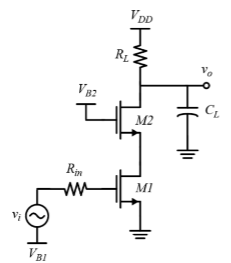
\includegraphics[width=0.3\textwidth]{q3.png}
\end{center}
\begin{align}
  g_{m} &= \qty{1}{\milli\siemens} \\
  r_{o} &= \qty{100}{\kilo\ohm} \\
  C_{gd} &= \qty{3}{\femto\farad} \\
  C_{sb} &= \qty{5}{\femto\farad} \\
  C_{db} &= \qty{4}{\femto\farad} \\
  R_{in} &= \qty{3}{\kilo\ohm} \\
  R_{L} &= \qty{2}{\kilo\ohm} \\
  C_{L} &= \qty{100}{\femto\farad}
\end{align}

\begin{subparts}
  \item
  Assuming a high enough frequency such that the capacitor impedances are much larger than any other impedances in the circuit, the small-signal model of M2 is
  \begin{center}
    \begin{circuitikz}\draw
      (0, 0) node[circ, label=above:\(G\)](g){}  to[open, v=\(v_{gs}\)] ++(0, -2) to[short] ++(4, 0) to[cI, l={\(g_{m} v_{gs}\)}, invert] ++(0, 2) to[short] ++(2, 0) coordinate(vd) to[R, l=\(r_{o2}\)] ++(0, -2) to[short] ++(-2, 0)
      (g)++(0, -2) node[circ, label=left:\(S\)]{} to[short] ++(2, 0) to[R, l=\(r_{o1}\)] ++(0, -2) node[ground]{}
      (g) to[short] ++(-1, 0) to[short] ++(0, -2) node[ground]{}
      (vd) to[short] ++(2, 0) to[sV, l=\(v_{t}\), i^=\(i_{t}\)] ++(0, -2) node[ground]{}
    ;\end{circuitikz}
  \end{center}
  The source voltage can be found as
  \begin{align}
    i_{t} &= \frac{v_{t} - v_{s}}{r_{o2}} - g_{m} v_{s} \\
    \frac{v_{t} - v_{s}}{r_{o2}} - g_{m} v_{s} &= \frac{v_{s}}{r_{o1}} \\
    \implies r_{o} (v_{t} - v_{s}) - g_{m} r_{o}^{2} v_{s} &= r_{o} v_{s} \\
    \implies v_{s} &= \frac{r_{o}}{2 r_{o} + g_{m} r_{o}^{2}} v_{t}
  \end{align}
  For M1, since both gate and source are grounded, we can ignore the transconductance, so we have that \(v_{s} = i_{t} r_{o}\), so
  \begin{equation}
    i_{t} \cancel{r_{o}} = \frac{\cancel{r_{o}}}{2 r_{o} + g_{m} r_{o}^{2}} v_{t} \implies \frac{v_{t}}{i_{t}} = g_{m} r_{o}^{2} + 2 r_{o} = \qty{10.2}{\mega\ohm}
  \end{equation}
  \item
  Assume a high enough frequency such that the capacitor impedances are much larger than any other impedances in the circuit.
  Since we are looking into the source of M2, we do not need to consider the effect of M1.
  Thus, the impedance is nothing more than the impedance of a common-gate amplifier, which is
  \begin{equation}
    R_{in} = \left(g_{m} \frac{1 + \frac{1}{g_{m} r_{o}}}{1 + \frac{R_{L}}{r_{0}}}\right)^{-1} = \qty{1010}{\ohm}
  \end{equation}
  \item
  Using the \(A_{v} = -G_{m} R_{o}\) method, we can find \(R_{o}\) as the result of the first part, and \(G_{m}\) can be found from discussion as
  \begin{equation}
    \frac{v_{o}}{v_{i}} = -g_{m} r_{o} \frac{R_{out} \parallel R_{L}}{r_{o} + R_{in}} = -1.98
  \end{equation}
  \item
  \begin{center}
    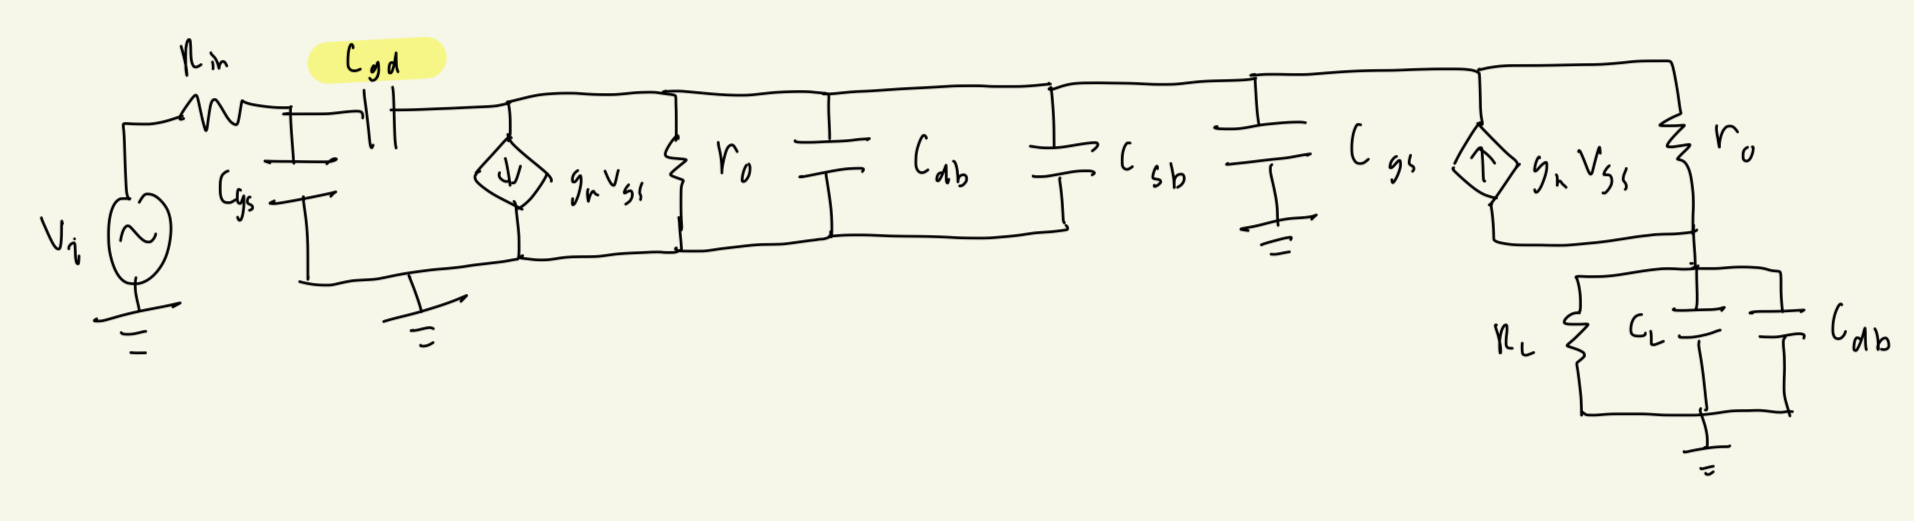
\includegraphics[width=0.9\textwidth]{q3d.png}
  \end{center}
  Note that we can combine many of the capacitances into their equivalences, such as the body capacitors in the middle and the capacitors at the drain of M2.
  \item
  \begin{center}
    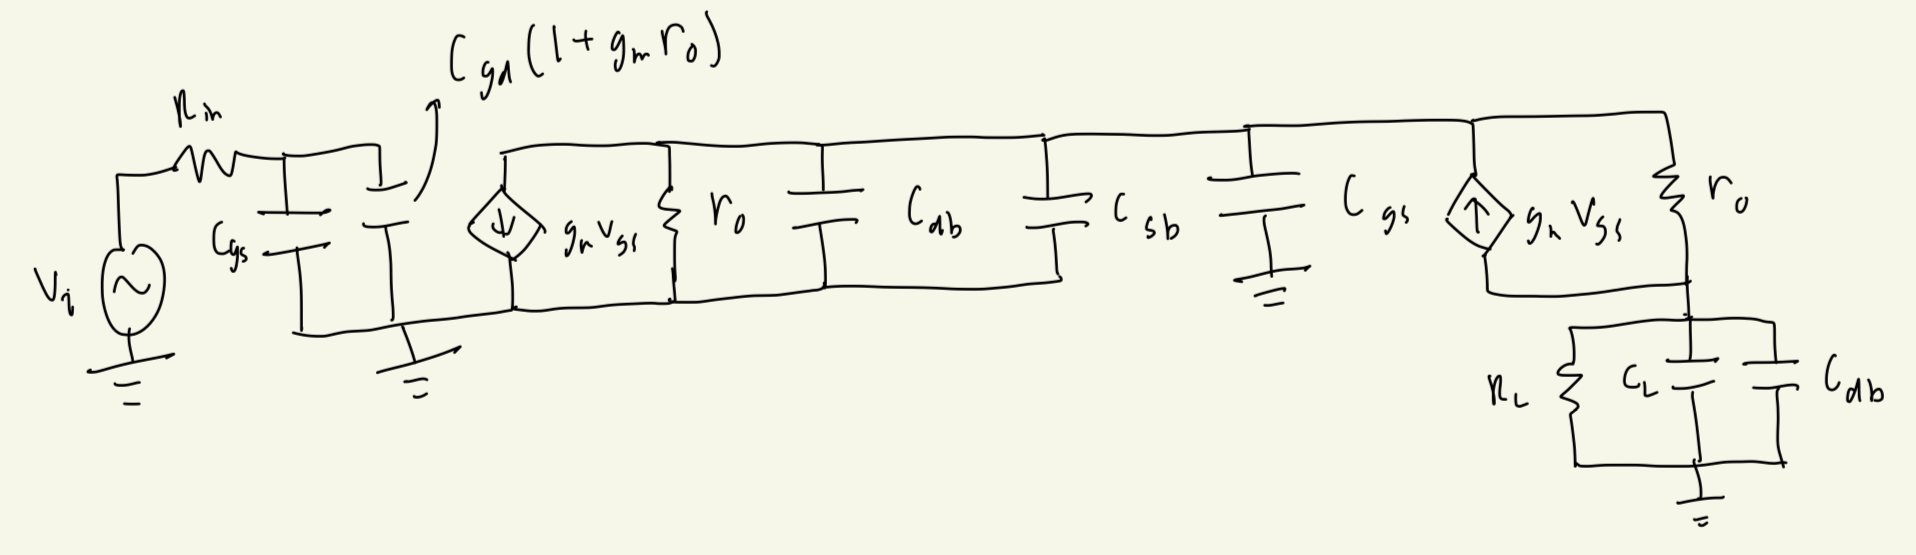
\includegraphics[width=0.9\textwidth]{q3e.png}
  \end{center}
  \item
  The second-stage amplifier is a common-drain amplifier.
  Since the gain of a common-drain amplifier is one, the low-frequency small-signal gain is unchanged, i.e.
  \begin{equation}
    \frac{v_{o}}{v_{i}} = -g_{m} r_{o} \frac{R_{out} \parallel R_{L}}{r_{o} + R_{in}} = -1.98
  \end{equation}
\end{subparts}

\end{document}
